\subsection{K-nearest neighbours}

The data set has been exposed to classification by looking at the k nearest neighbours.

\begin{figure}[H]
	\begin{subfigure}[b]{0.5\textwidth}
	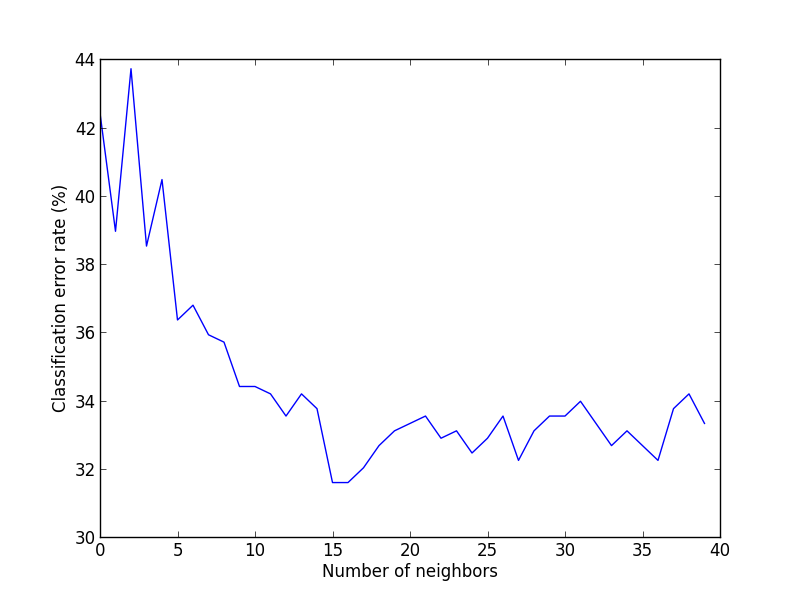
\includegraphics[scale=0.3]{pictures/knnX.png}
	\caption{Looking at all attributes.}
	\label{knnResultX}
	\end{subfigure}
	\begin{subfigure}[b]{0.5\textwidth}
	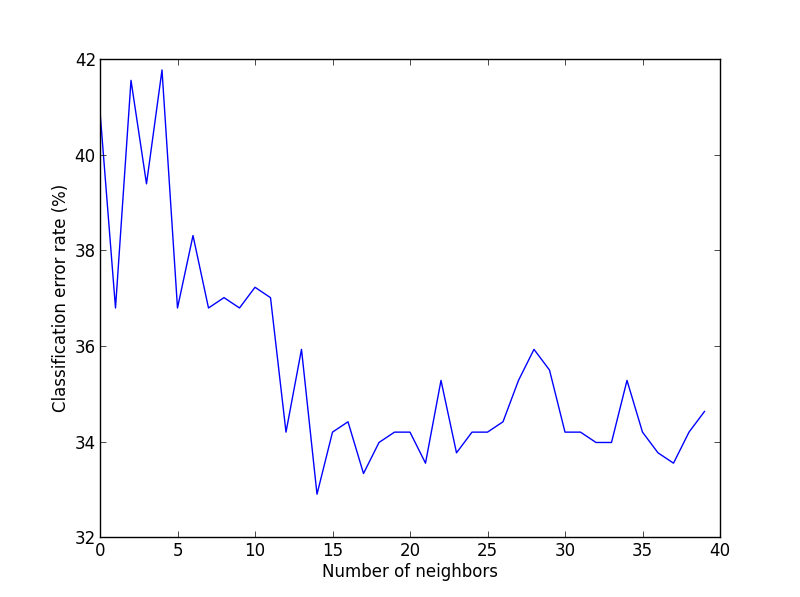
\includegraphics[scale=0.3]{pictures/knnXAD.png}	
	\caption{Looking at attributes selected by forward selection.}
	\label{knnResultXad}
	\end{subfigure}

	\begin{subfigure}[b]{0.5\textwidth}
	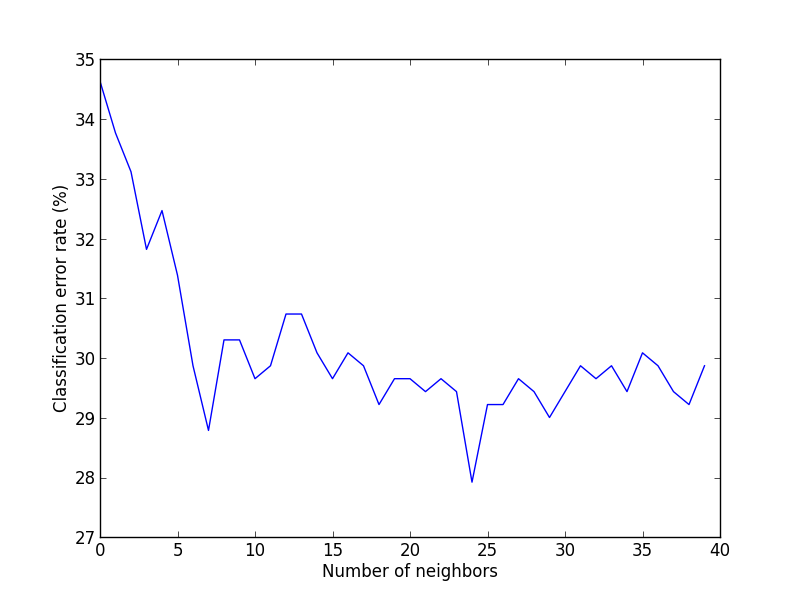
\includegraphics[scale=0.3]{pictures/knnPC.png}
	\caption{Looking at all principal components.}
	\label{knnResultXPA}
	\end{subfigure}
	\begin{subfigure}[b]{0.5\textwidth}
	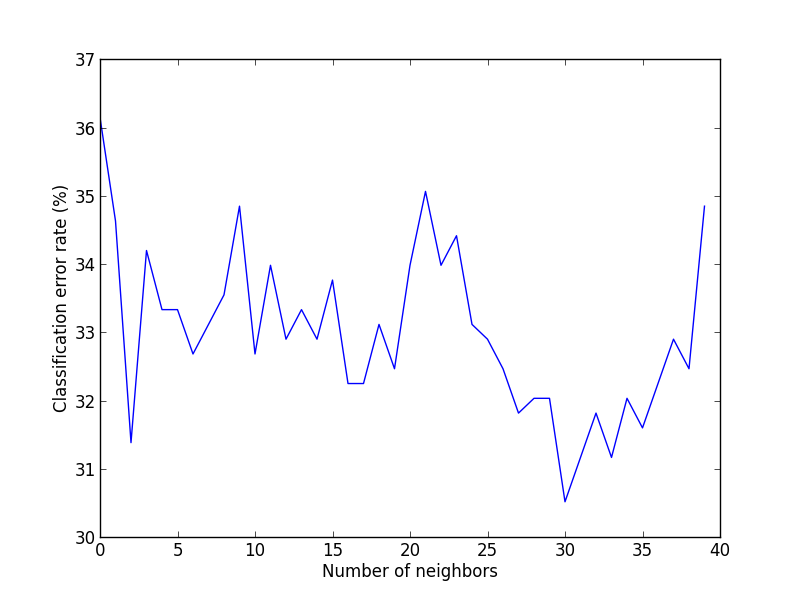
\includegraphics[scale=0.3]{pictures/knn2PC.png}
	\caption{Looking at two most important principal components.}
	\label{knnResultX2PA}
	\end{subfigure}
\caption{These figure shows results of performing KNN for different input.}
\label{knnResults}
\end{figure}

The misclassification rates for these can be seen in Table \ref{knnErrorRate}.

\begin{table}[H]
\begin{longtable}{lc} \hline
Result from: & Mis-classification rate \\ \hline
Figure \ref{knnResultX} & 32\% \\ 
Figure \ref{knnResultXad} & 33\% \\ 
Figure \ref{knnResultXPA} & 28\% \\ 
Figure \ref{knnResultX2PA} & 30,5\% \\ \hline
\end{longtable}
\caption{Mis-classification rate for the logistic regressions.}
\label{knnErrorRate}
\end{table}

%The first figure shows the estimated error using all available attributes. The lowest error of 32\% is found when using 15 nearest neighbours.

%The next figure shows the estimated error using only the selected attributes from the forward selection done in the linear regression analysis. This indicates a slightly higher estimated error of 33\%, using 14 neighbours.

%The next figure uses all the principal components. This indicates a lower estimated error of around 28\%, using 24 neighbours.

%The last figure uses only the two most important principal components. This gives an error of 30.5\% using 30 neighbours.

\begin{figure}[H]
	\begin{subfigure}[b]{0.5\textwidth}
	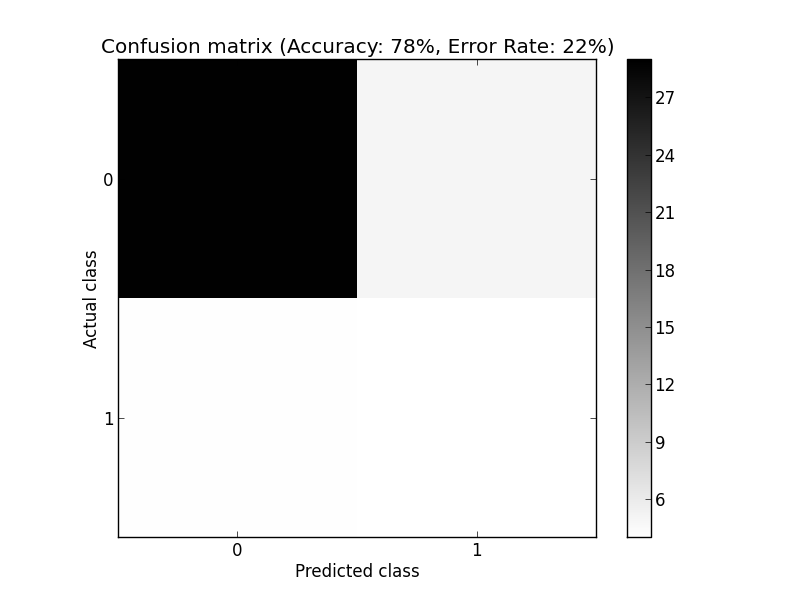
\includegraphics[scale=0.2]{pictures/cmX.png}
	\caption{Looking at all attributes. \newline Giving an accuracy of 78\% }
	\label{cmResultX}
	\end{subfigure}
	\begin{subfigure}[b]{0.5\textwidth}
	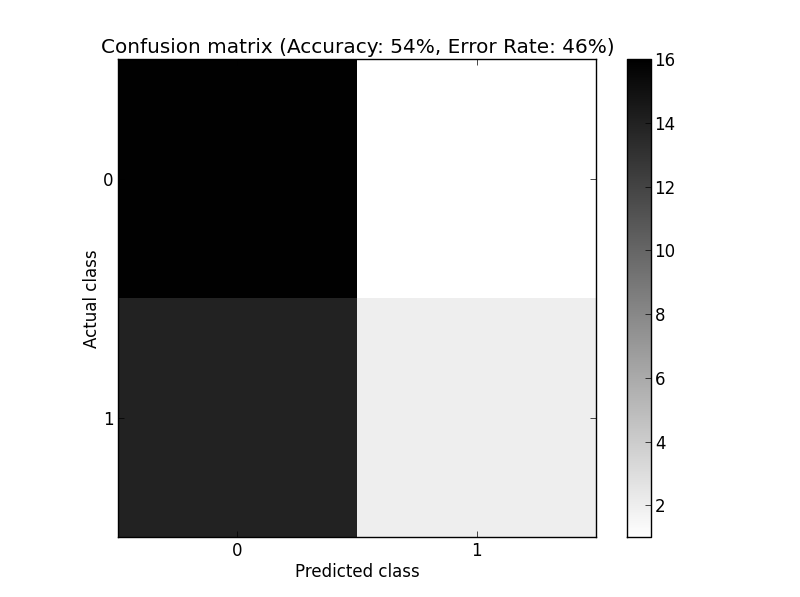
\includegraphics[scale=0.2]{pictures/cmXAD.png}	
	\caption{Looking at attributes selected by forward selection.  Giving an accuracy of 54\%}
	\label{cmResultXad}
	\end{subfigure}

	\begin{subfigure}[b]{0.5\textwidth}
	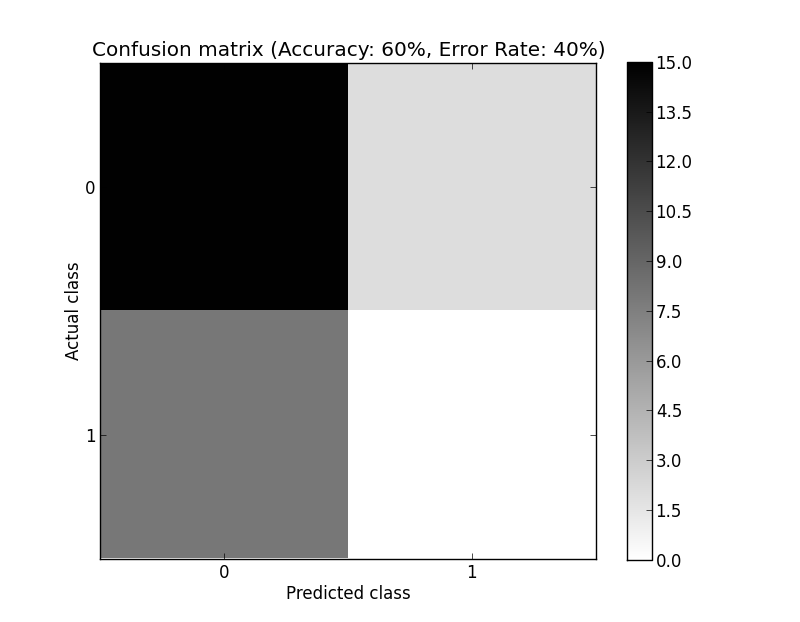
\includegraphics[scale=0.2]{pictures/cmPC.png}
	\caption{Looking at all principal components. \newline Giving an accuracy of 72\%}
	\label{cmResultXPA}
	\end{subfigure}
	\begin{subfigure}[b]{0.5\textwidth}
	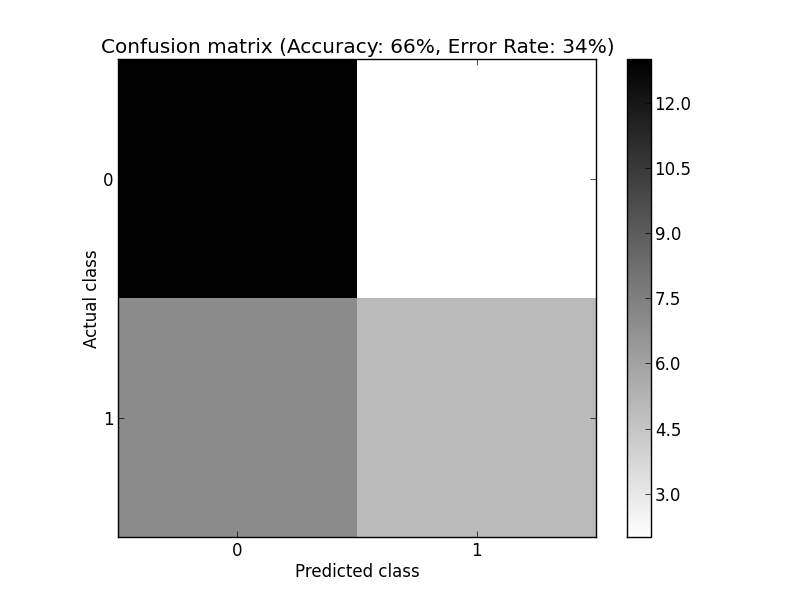
\includegraphics[scale=0.2]{pictures/cm2PC.png}
	\caption{Looking at two most important principal components.  Giving an accuracy of 66\%}
	\label{cmX2PA}
	\end{subfigure}
\caption{This figure shows results of doing a confusion matrix for different inputs}
\label{cmResults}
\end{figure}
The above confusion matrixes shows the accuracy and error rate for the K-Nearest Neighbours performed before.

